\section{WrapperException}\label{code:WrapperException}
The class \lstinline|WrapperException| is described in chapter \tqfullvref{sec:DomainSpecificExceptions}. It is meant as the base class for a hierarchy of domain specific exceptions.

\begin{center}
% Generated by "dot -Tpng -y WrapperException.gv > WrapperException.png"
	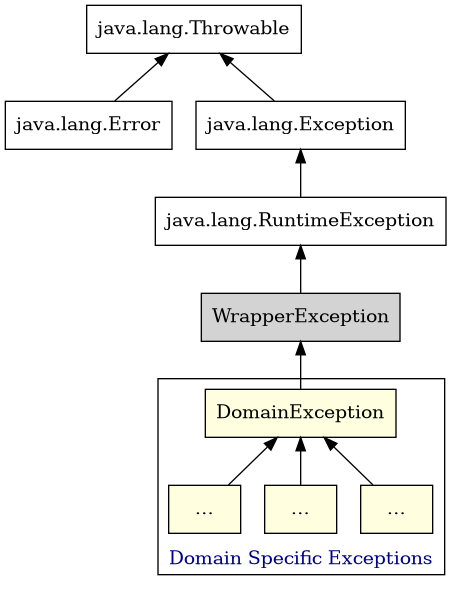
\includegraphics[scale=0.6]{code/WrapperException}
\end{center}

A real life implementation can be found at \autocite{TQUADRAT_ORG_FOUNDATION_WRAPPEREXCEPTION}.

The \lstinline|DomainException| shown on the next page is an example for a domain specific root exception that is used as a container for other exceptions.

\clearpage

\begin{lstlisting}
/**
 *  <p>{@summary An implementation of
 *  {@link WrapperException}
 *  as the domain specific root exception.}</p>
 *  <p>This implementation is a pure container exception.</p>
 */
public class DomainException extends WrapperException
{
        /*--------------*\
    ====** Constructors **================================================
        \*--------------*/
    /**
     * <p>{@summary Constructs a new instance of {@code DomainException}
     * with the specified detail message and
     * cause.}</p>
     *
     * @param message The detail message that is saved for later
     *     retrieval by the
     *     {@link #getMessage()}
     *     method.
     * @param cause The cause that is saved for later retrieval by the
     *     {@link #getCause()}
     *     method.
     */
    public DomainException( final String message, final Throwable cause ) 
    { 
        super( message, cause, false ); 
    }   //  WrapperTestException()

    /**
     * <p>{@summary Constructs a new instance of {@code DomainException}
     * that wraps the specified cause.}</p>
     *
     * @param cause The cause that is saved for later retrieval by the
     *     {@link #getCause()}
     *     method.
     */
    public DomainException( final Throwable cause ) 
    { 
        super( null, cause, false );
    }   //  WrapperTestException()

    /**
     * <p>{@summary Constructs a new instance of {@code DomainException}
     * with the specified detail message, cause, and whether the stack
     * trace should be retrieved.}</p>
     * <p>If {@code retrieveStacktrace} is {@code false}, the instance is
     * a pure wrapper or container for other exceptions; consequently
     * {@code cause} cannot be {@code null} if {@code retrieveStacktrace}
     * is {@code false}. In that case, if {@code cause} is an instance of
     * {@code WrapperException}, it will be replaced by
     * {@linkplain Throwable#getCause() its cause}
     * if that is not {@code null}. In that case, the additional
     * information is merged, too.</p>
     * <p>If {@code message} is {@code null} and {@code cause} is an
     * instance of {@code WrapperException}, the internal message of
     * {@code cause} is used instead.</p>
     * <p>If {@code message} is {@code null} and {@code cause} is another
     * exception type, the result of
     * {@link Throwable#toString() cause::toString}
     * is used as the detailed message for the new instance.</p>
     *
     * @param message The detail message that is saved for later
     *     retrieval by the
     *     {@link #getMessage()}
     *     method. It can be {@code null}.
     * @param cause The cause that is saved for later retrieval by the
     *     {@link #getCause()}
     *     method. It can be {@code null}.
     * @param retrieveStacktrace {@code true} if the stack trace will be
     *     retrieved and is writable and the instance should behave like
     *     a <i>regular</i> exception, {@code false} if the instance
     *     should be a pure container.
     */
    protected DomainException( final String message, final Throwable cause, final boolean retrieveStacktrace )
    {
        super( message, cause, retrieveStacktrace );
    }   //  DomainException()
}
//  class DomainException
\end{lstlisting}

The other exceptions of that hierarchy would be similar like the below shown \lstinline|ProcessingException|:
\begin{lstlisting}
/**
 * <p>{@summary The exception that is thrown by methods from this
 * domain in case a processing problem surfaced.} It is an implementation
 * of
 * {@link WrapperException},
 * derived from
 * {@link DomainException}.</p>
 */
public class ProcessingException extends DomainException
{
        /*--------------*\
    ====** Constructors **================================================
        \*--------------*/
    /**
     * <p>{@summary Constructs a new instance of
     * {@code ProcessingException} without a detail message and a
     * cause.}</p>
     */
    public ProcessingException()
    {
        super( null, null, true );
    }   //  ProcessingException

    /**
     * <p>{@summary Constructs a new instance of
     * {@code ProcessingException} with the specified detail message and
     * cause.}</p>
     *
     * @param message The detail message that is saved for later
     *     retrieval by the
     *     {@link #getMessage()}
     *     method.
     * @param cause The cause that is saved for later retrieval by the
     *     {@link #getCause()}
     *     method.
     */
    public ProcessingException( final String message, final Throwable cause )
    {
        super( message, cause, true );
    }   //  ProcessingException

    /**
     * <p>{@summary Constructs a new instance of
     * {@code ProcessingException} that wraps the specified cause.}</p>
     *
     * @param cause The cause that is saved for later retrieval by the
     *     {@link #getCause()}
     *     method.
     */
    public ProcessingException( final Throwable cause )
    {
        super( null, cause, true );
    }   //  ProcessingException

    /**
     * <p>{@summary Constructs a new instance of {@code ProcessingException}.}
     * <p>For the details, refer to
     * {@link DomainException#DomainException(String,Throwable,boolean)}.</p>
     *
     * @param message The detail message. It can be {@code null}.
     * @param cause The cause. It can be {@code null}.
     * @param retrieveStacktrace {@code true} if the stack trace will be
     *     retrieved and is writable and the instance should behave like
     *     a <i>regular</i> exception, {@code false} if the instance
     *     should be a pure container.
     */
    protected DomainException( final String message, final Throwable cause, final boolean retrieveStacktrace )
    {
        super( message, cause, retrieveStacktrace );
    }   //  DomainException()
}
//  class ProcessingException

/*
 *  End of File
 */
\end{lstlisting}

When the exception class is final, the protected constructor\index{constructor} in line~67 is obsolete and should be omitted.

%------------------------------------------------------------------------------

\paragraph{The Code} \
\lstinputlisting[caption={WrapperException.java}]{coding/customExceptions/WrapperException.java}

%==============================================================================
% End of file!!
%==============================================================================

